\documentclass[a4paper]{article}

\usepackage[utf8]{inputenc}
\usepackage[english]{babel}
\usepackage{fancyhdr,graphicx}
\usepackage[colorlinks=true,linkcolor=black,urlcolor=blue,bookmarksopen=true]{hyperref}

\newcommand{\materia}{[75.41] Taller de Programación I}
\newcommand{\trabajo}{Documentación técnica}
\newcommand{\trabajoheader}{Ejercicio final }
\newcommand{\cuatri}{1c2019}
\newcommand{\cuatrimestre}{Primer cuatrimestre de 2019}
\newcommand{\grupo}{Grupo 3}

\newcommand{\autores}{
	Camila Bojman,
	Cecilia Hortas,
	Nicolas Vazquez}

\hypersetup{
	pdftitle={\trabajo},
	pdfsubject={\materia},
	pdfauthor={\autores},
}

\pagestyle{fancy}
\fancyhf{}
\fancyhead[L]{\materia}
\fancyhead[R]{\trabajoheader - \trabajo}
\renewcommand{\headrulewidth}{0.4pt}
\fancyfoot[C]{\thepage}
\renewcommand{\footrulewidth}{0.4pt}

\begin{document}
	\pagenumbering{gobble}
	\pagenumbering{roman}
	\pagenumbering{arabic}
	\setcounter{page}{1}
	
	\begin{titlepage}
		\hfill
\includegraphics[width=6cm]{fiuba.jpeg}
		\begin{center}
			\vfill
			\Huge \textbf{\trabajo}
			\vskip2cm
			\Large \materia\\
			\cuatrimestre
			\vfill
			\grupo
			\begin{itemize}
				\item Camila Bojman 101055 camiboj@gmail.com
				\item Cecilia Hortas 100687 ceci.hortas@gmail.com
				\item Nicolas Vazquez 100338 vazquez.nicolas.daniel@gmail.com
			\end{itemize}
			\vskip1cm
		\end{center}
	\end{titlepage}

\section{Requerimientos de software}

En primer lugar el programa fue desarrollado enteramente en C++ en un sistema operativo Linux por lo que los comandos que se detallarán a continuación son para ese sistema operativo y sus distribuciones afines. Las bibliotecas utilizadas se presentan a continuación:

\begin{itemize}
	\item \texttt{Box 2D}: se encuentra en el repositorio por lo que basta con clonar el mismo
\end{itemize}

\begin{itemize}
	\item \texttt{Native JSON Benchmark}: igualmente se encuentra en el repositorio
\end{itemize}

\begin{itemize}
	\item \texttt{SDL}: se debe instalar a partir de los siguientes comandos:
\end{itemize}

\begin{verbatim}
sudo apt-get install libsdl2-dev
sudo apt-get install libsdl2-image-dev
\end{verbatim}

\begin{itemize}
	\item \texttt{SDL-mixer}: se debe instalar a partir del siguiente comando:
\end{itemize}

\begin{verbatim}
sudo apt-get install libsdl2-mixer-dev
\end{verbatim}

\begin{itemize}
	\item \texttt{YAML}: se debe instalar a partir del siguiente comando:
\end{itemize}

\begin{verbatim}
sudo apt-get install libyaml-cpp-dev
\end{verbatim}

\begin{itemize}
	\item \texttt{TTF}: se debe instalar a partir del siguiente comando:
\end{itemize}

\begin{verbatim}
sudo apt-get install libsdl2-ttf-dev
\end{verbatim}

\begin{itemize}
	\item \texttt{ffmpeg}: se debe instalar a partir de los siguientes comandos:
	
\begin{verbatim}
	sudo apt install libavutil libswresample libavformat libavcodec
	sudo apt-get install ffmpeg
\end{verbatim}
\end{itemize}

\begin{itemize}
	\item \texttt{CMake}: se debe instalar a partir de los siguientes comandos:
	\footnote{Fuente: https://askubuntu.com/questions/355565/how-do-i-install-the-latest-version-of-cmake-from-the-command-line}
	
	\begin{enumerate}
		\item Desinstalar cualquier versión previa de CMake:
		\begin{verbatim}
		sudo apt remove --purge --auto-remove cmake
		\end{verbatim}
		\item Ir a la página oficial de CMake y bajar la última versión: 
		\begin{verbatim}
		http://www.cmake.org/download
		\end{verbatim}
		\item Correr los siguientes comandos:
		\begin{verbatim}
		$ version=3.14
		$ build=5
		$ mkdir ~/temp
		$ cd ~/temp
		$ wget https://cmake.org/files/v$version/cmake-$version.$build.tar.gz
		$ tar -xzvf cmake-$version.$build.tar.gz
		$ cd cmake-$version.$build/
		$ ./bootstrap
		$ make -j4
		$ sudo make install
		\end{verbatim}
		\item Verificar la versión de CMake:
		\begin{verbatim}
		$ cmake --version
		cmake version 3.14.X
		\end{verbatim}
	\end{enumerate}
\end{itemize}

\subsection{Instalación}
En el \texttt{root} del repositorio clonado se encuentra un archivo \texttt{install.sh}. Para realizar la instalación se deben seguir los siguientes pasos:

\begin{verbatim}
chmod +x install.sh
./install.sh <path>
\end{verbatim}
donde \texttt{<path>} es el directorio donde se desea instalar el juego.

Para proceder a jugar al juego se deben seguir los siguientes pasos:

\begin{enumerate}
	\item Levantar un servidor con el comando \texttt{./Server <port>}
	\item Conectarse con el cliente con \texttt{./Client <host> <port>} siendo \texttt{<host>} una dirección IP y \texttt{<port>} el mismo puerto del servidor.
\end{enumerate}

Para crear y editar mapas, ejecutar \texttt{./Editor}.

\section{Descripción general}

El proyecto se constituye de los siguientes módulos:

\begin{itemize}
	\item \textbf{Servidor}

Se encuentran tanto las clases designadas al soporte físico del juego como al soporte multijugador y multipartida.

	\item \textbf{Cliente gráfico}
	
Se encuentran las clases designadas para modelar el cliente desde un lado gráfico con el uso de la librería \texttt{SDL} así como el soporte para manejar la recepción del estado actual del escenario para dibujarlo y el envío de los diversos eventos de usuarios para que sean modelados por el motor físico.
	\item \textbf{Editor}
	
Se encuentran las clases designadas para el modelado del editor que se tratan escencialmente de \textit{wrappers} de diversas funcionalidades de \texttt{SDL} y \texttt{ffmpeg}.

	\item \textbf{Archivos compartidos}
	
Se tratan de diversas clases que se consideró que podían ser útiles para más de un módulo por lo que se colocaron en un espacio común para su correcta compilación.
\end{itemize}

\section{Archivos compartidos}

Se tratan de clases que no necesariamente están relacionadas entre sí por lo que se considera que no es pertinente a la documentación exponer un diagrama de clases. Sin embargo, sí se mostrará su relación con las futuras clases. De esta forma, las principales clases que componen este módulo son:

\newpage

\begin{itemize}
	\item \textbf{Socket}
\end{itemize}

Esta clase encapsula todas las operaciones realizadas para la comunicación a través de un socket.

\begin{itemize}
	\item \textbf{Protocol}
\end{itemize}

Esta clase encapsula el protócolo utilizado para el desarrollo del juego. Contiene una referencia a un \texttt{Socket} y modela el envío y recepción de \texttt{strings}.

\begin{itemize}
	\item \textbf{Thread}
\end{itemize}

Esta clase encapsula el funcionamiento de un thread. Su principal atributo es una variable de tipo \texttt{std::thread} a la que se le pasa como parámetro una
referencia a la función \texttt{run()} que encapsula la ejecución.

\begin{itemize}
	\item \textbf{UserEventQueue}
\end{itemize}

Se trata de una cola bloqueante a la que se encola los diversos eventos de usuarios que deben ser modelados por el motor físico.

\begin{itemize}
	\item \textbf{StageStatusQueue}
\end{itemize}

Se trata de una cola bloqueante a la que se encola el estado del escenario en un step dado por el escenario para que sea dibujado por los diversos clientes.

\begin{itemize}
	\item \textbf{Window}
\end{itemize}

Se trata de una clase wrapper de \texttt{SDL\_Window} y \texttt{SDL\_Renderer}. Se utiliza en absolutamente todas las vistas y operaciones que requieran dibujar a pantalla.
La clase fue protegida debido a que ha de ser compartida entre el hilo que procesa input de usuario y el hilo que dibuja, para poder manejar el cambio de tamaño de la pantalla de Fullscreen a Windowed y viceversa.

\begin{itemize}
	\item \textbf{SDLSession}
\end{itemize}

Se trata de una clase wrapper de la inicialización de los distintos módulos de SDL. Se utiliza en el Cliente y en el Editor.

\begin{itemize}
	\item \textbf{Sprite}
\end{itemize}

Se trata de una clase wrapper para la carga de texturas en SDL.

\begin{itemize}
	\item \textbf{AnimatedSprite}
\end{itemize}

Se trata de una clase wrapper para mostrar animaciones por pantalla. Utiliza tiras de sprites cargadas en un Sprite para poder dibujar cada cuadro de la tira de sprites cada cierto tiempo.
Cuenta con un timer para determinar cada cuánto tiempo hay que actualizar el cuadro actual que será dibujado en el loop principal del juego.

\section{Servidor}

\subsection{Descripción general}
Las funcionalidades del servidor se dividen en dos partes:
\begin{enumerate}
	\item Las relativas al motor físico, es decir, el modelado físico del juego.
	\item Las relativas al manejo de threading y sockets para brindar un soporte multijugador y multipartida.
\end{enumerate}

A continuación se enumeran las principales clases que se encargan de implementar dichas funcionalidades y sus principales atributos y métodos.

\subsection{Clases}

Para describir las clases utilizadas se dividirán las clases en 5 categorías:
\begin{itemize}
	\item Soporte de comunicación (threading y sockets)
	\item Entidades del juego
	\item Manejo de portales
	\item Manejo del escenario
	\item Movimientos del juego
\end{itemize} 

\subsubsection{Soporte de comunicación}

Estas clases se realizaron para modelar la comunicación con el cliente. Son las que encapsulan la comunicación por medio de sockets y el manejo de threads para brindar el soporte multipartida y multijugador del juego.

\begin{itemize}
	\item \textbf{Stage Manager}
\end{itemize}

Se encarga de controlar todo lo relativo al escenario y la partida a crear. Tiene como principales atributos una cantidad máxima de jugadores, una referencia al escenario de partida, un parser que se encarga de manejar el archivo \texttt{YAML} que contiene la información de los niveles a utilizar, una cola de eventos y una cola de clientes que contiene el estado actual de los mapas.  Cabe destacar que esta clase es la que se encarga de manejar los eventos de usuario y traducirlos a eventos en el mundo físico.

\begin{itemize}
	\item \textbf{Room Worker}
\end{itemize}

Esta clase se encarga de manejar la creación y la unión de partidas. Por lo tanto, es necesario que mantenga una referencia al socket del cliente, a su respectivo protocolo que encapsula la comunicación y a la clase \texttt{Room Manager} que se encarga de brindar los recursos necesarios para llevar esto a cabo.

\begin{itemize}
	\item \textbf{Room Manager}
\end{itemize}

Esta clase se encarga de organizar las diversas partidas creadas, agregar los jugadores a las mismas y remover las partidas que finalizaron.

\begin{itemize}
	\item \textbf{Room Acceptor}
\end{itemize}

Esta clase se utiliza para encapsular la aceptación de los clientes al servidor por lo que tiene como principal atributo un vector de punteros a la clase \texttt{Room Worker} para lanzarlos con el método \texttt{start} para inicializar los threads.

\begin{itemize}
	\item \textbf{Client Sender}
\end{itemize}

Esta clase se encarga de mandar a los clientes el estado actual del mundo físico por lo que sus atributos son referencias al socket del cliente y su protocolo así como una cola que guarda el estado actual del escenario.

\begin{itemize}
	\item \textbf{Client Receiver}
\end{itemize}

Esta clase se encarga de recibir los eventos de usuario para luego manejarlos por lo que mantiene una referencia al socket del cliente y una cola de eventos de usuario para encolar la serie de eventos recibidos.

\begin{itemize}
	\item \textbf{Client Handler}
\end{itemize}

Esta clase se encarga de manejar e inicializar las clases \texttt{Client Sender} y \texttt{Client Receiver} por lo que debe tener como atributos una referencia al socket del cliente y tanto una cola de eventos de usuario como una cola de estados actuales del escenario.
	
\subsubsection{Entidades del juego}

Se realizó una clase para cada elemento del juego de manera de modelizar sus responsabilidades y además se agregaron otras clases para hacer uso del polimorfismo y herencia de C++.

Es pertinente aclarar como elemento base del modelo que se utiliza una clase \texttt{Entity} de la cual derivan todas las clases de esta sección para poder modelizar las colisiones entre objetos. De esta manera, en caso de ocurrir una colisión, siempre sucede entre dos objetos de la clase \texttt{Entity} y por medio de la herencia se pudo manejar cada caso en particular con la sobreescritura de un método llamado \texttt{handleCollisions}. 

\begin{itemize}
	\item \textbf{Entity}
\end{itemize}

Tiene como atributos un string que denota el tipo de objeto y un puntero a un objeto de tipo \texttt{b2Body} de la libería Box2D. Tiene el método virtual puro \texttt{void handleCollision(Entity* entity)} para que lo implementen las clases derivadas y hagan un correcto manejo de colisiones.

\begin{itemize}
	\item \textbf{Acid}
\end{itemize}

Su principal método consiste en contempla las colisiones con instancias de la clase \texttt{Chell} ya que debe matarla.

\newpage
\begin{itemize}
	\item \textbf{Shot}
\end{itemize}

Esta clase se encarga de modelizar el disparo. Tiene como atributos dos punteros a la clase \texttt{Coordinate} (que representa una coordenada) tanto para el origen como el destino del disparo, un booleano que indica si finalizó el recorrido, un ángulo de disparo y un puntero a la clase \texttt{Chell} para poder asignarle los portales creados a la misma.

\begin{itemize}
	\item \textbf{Blue Shot}
\end{itemize}

Esta clase hereda de la clase \texttt{Shot} y maneja la colisión con un bloque de metal ya que debe crear un portal sobre el mismo de color azul.

\begin{itemize}
	\item \textbf{Orange Shot}
\end{itemize}

Esta clase hereda de la clase \texttt{Shot} y maneja la colisión con un bloque de metal ya que debe crear un portal sobre el mismo de color naranja.

\begin{itemize}
	\item \textbf{Cake}
\end{itemize}

Esta clase principalmente maneja las colisiones con objetos de la clase \texttt{Chell} ya que debe ganar en caso de colisionar.

\begin{itemize}
	\item \textbf{Chell}
\end{itemize}

Esta clase tiene como atributos un puntero al objeto que alberga el portal naranja, otro al objeto que alberga el portal azul y dos punteros a la clase \texttt{Coordinate} que representan los dos portales a teletransportarse. Además guarda un puntero a la clase \texttt{PinTool} y a la clase \texttt{Rock} en caso de estar agarrando una roca. Sus principales métodos implican moverse a la derecha, moverse a la izquierda, saltar, agarrar una roca y dejarla, agregar los portales una vez realizados y contemplar los diversos casos de colisión con el resto de los objetos,

\begin{itemize}
	\item \textbf{Diagonal Metal Block}
\end{itemize}

Esta clase tiene como atributo el ángulo de rotación para representar los cuatro bloques en diagonal y su principal método consiste en manejar las colisiones con los objetos de la clase \texttt{Energy Ball} para que cambie su dirección en caso de colisionar.

\begin{itemize}
	\item \textbf{Metal Block}
\end{itemize}

Esta clase tiene como responsabilidad principal manejar las colisiones con las bolas de energía para invertir su sentido y además con los disparos \texttt{Blue Shot} y \texttt{Orange Shot} para generar los portales.

\begin{itemize}
	\item \textbf{Rock Block}
\end{itemize}

Esta clase se encarga principalmente de manejar las colisiones con las bolas de energía para que desaparezcan y con los disparos para no generar portales en caso de colisionar.

\newpage

\begin{itemize}
	\item \textbf{Energy Ball}
\end{itemize}

Esta clase tiene como método principal el que consiste en volar de acuerdo a la dirección establecida por el emisor de energía y además cambiar su dirección en caso de colisionar con un objeto de la clase \texttt{Diagonal Block} o rebotar en caso de colisionar con un objeto de la clase \texttt{Metal Block}.

\begin{itemize}
	\item \textbf{Energy Transmitter}
\end{itemize}

Esta clase se encarga principalmente de controlar la frecuencia de lanzamiento de las bolas de energía. De esta clase derivan las otras cuatro clases que designan las cuatro direcciones posibles que pueden tomar las bolas de energía (arriba, abajo, izquierda o derecha).

\begin{itemize}
	\item \textbf{Energy Bar}
\end{itemize}

Esta clase principalmente maneja las colisiones con los disparos y con las rocas para evitar el traspaso de las mismas.


\begin{itemize}
	\item \textbf{Gate}
\end{itemize}

Esta clase tiene como atributos un string que designa la lógica que debe seguirse para abrir la puerta y además un mapa que guarda los distintos botones involucrados en dicha lógica con su id como clave y un puntero al objeto \texttt{Button} como valor. Su principal método es el encargado de determinar si la puerta está abierta o cerrada de acuerdo al estado actual de los botones (encendido y apagado).

\begin{itemize}
	\item \textbf{Item Activable}
\end{itemize}

Esta clase fue implementada para que los dos objetos que pueden ser encendidos del escenario puedan heredar de ella. Por lo tanto, sus principales métodos consisten en activarlos, desactivarlos y determinar su estado.

\begin{itemize}
	\item \textbf{Button}
\end{itemize}

Esta clase hereda de la clase \texttt{Item Activable}. Su principal método consiste en manejar las colisiones con los objetos de la clase \texttt{Chell} y \texttt{Rock} para poder determinar su estado (encendido u apagado), guardado como atributo.

\begin{itemize}
	\item \textbf{Energy Receptor}
\end{itemize}

Esta clase hereda de la clase \texttt{Item Activable}. Su principal método consiste en manejar las colisiones con los objetos de la clase \texttt{Energy Ball} para poder determinar su estado (encendido u apagado), guardado como atributo.

\begin{itemize}
	\item \textbf{Portal}
\end{itemize}

Esta clase tiene como atributo un enum de tipo \texttt{Orientation} que designa la orientación vertical u horizontal del portal y un enum de tipo \texttt{Direction} que designa la dirección en que deben salir los objetos al teletransportarse por el otro portal, es decir, izquierda, derecha, abajo o arriba. Se encarga de manejar las colisiones con los objetos de la clase \texttt{Chell}, \texttt{Energy Ball} y \texttt{Rock} para que se teletransporten al topar con un portal.

\begin{itemize}
	\item \textbf{Rock}
\end{itemize}

Esta clase tiene como atributos un booleano que designa si está vivo o muerto y otro para designar si está siendo agarrado o no por Chell. Su principal método consiste en manejar las colisiones con los diversos objetos del mundo, por ejemplo, un objeto de la clase \texttt{Button} para activarlo, de la clase \texttt{Chel}l para matarla si está por encima de ella y morir en caso de topar con un objeto de la clase \texttt{Energy Bar}.

\begin{itemize}
	\item \textbf{PinTool}
\end{itemize}

Esta clase tiene como método principal el que consiste en eliminar el objeto del escenario luego de pasado cierto tiempo predefenido.

\subsubsection{Manejo de portales}

Esta sección tiene las clases que se utilizan para designar los portales en el escenario. Es necesario seguir una cierta organización para unir los portales a un objeto de la clase \texttt{Chell} en particular, borrar un portal de un color en caso de crearse otro del mismo color y resetear los portales (borarlos del escenario). Las clases que se encargan de dichas responsabilidades son las que siguen:

\begin{itemize}
	\item \textbf{Portal Holder}
\end{itemize}

Esta clase guarda como atributos un puntero a la clase \texttt{Coordinate} que representa las coordenadas de un portal, un enum \texttt{Orientation} que designa su orientación (vertical u horizontal) y un enum \texttt{Direction} que indica para donde deben teletransportarse los objetos en caso de toparse con su portal contrario.

\begin{itemize}
	\item \textbf{Portal Manager}
\end{itemize}

Esta clase tiene como atributos una referencia a un \texttt{unordered\_map} que tiene como claves los ids como string de los portales y como valor un puntero al objeto de la clase \texttt{Portal}, además de una referencia al objeto de clase \texttt{Stage}. De esta manera se encarga de eliminar los portales del mundo y de crearlos de acuerdo a los portales actuales de la clase \texttt{Chell}.

\subsubsection{Manejo del escenario}

Estas clases son las encargadas de la organización global de los objetos en el escenario, su disposición en el escenario y su representación en \texttt{Box2D}.

\begin{itemize}
	\item \textbf{Coordinates}
\end{itemize}
Esta clase guarda dos atributos de tipo \texttt{float} que representan las coordenadas \texttt{x} e \texttt{y}.

\begin{itemize}
	\item \textbf{Physics World}
\end{itemize}
Esta clase se encarga de encapsular la creación de objetos en el mundo de \texttt{Box2D}. Por eso sus atributos son un puntero a un objeto de tipo \texttt{b2World} y el ancho y el largo del escenario como \texttt{floats}. Los principales métodos consisten en agregar rectángulos estáticos y dinámicos al escenario, triángulos estáticos y el caso particular para el objeto de la clase \texttt{Chell}: un rectangulo con dos ruedas en su parte inferior. Esto tuvo que realizarse para evitar que el objeto se trabe en los diversos rectángulos simulados como piso. Además, se encarga de la correcta destrucción de los objetos en el mundo y de simular el \textit{step} de \texttt{Box2D}.

\begin{itemize}
	\item \textbf{Stage}
\end{itemize}

Esta clase tiene como atributos una serie de \texttt{unordered\_map} donde se guardan todos los objetos del mundo como valor y como clave un id de clase \texttt{string} o un objeto de la clase \texttt{Coordinate} para el caso de los bloques estáticos. Su principal método es el que simula el \texttt{step} y llama a los diversos métodos que deben convocarse en cada llamada a la modelación del mundo físico. Además tiene un método que devuelve el \texttt{json} necesario para actualizar las vistas de los diversos clientes.

\begin{itemize}
	\item \textbf{Yaml Parser}
\end{itemize}
Esta clase es la encargada de unir el editor y el servidor. Tiene como atributos un nodo \texttt{YAML} y una referencia al \texttt{Stage}. De esta manera, lee el archivo \texttt{YAML} generado por el editor, agrega los objetos que debe agregar al escenario y genera los \texttt{json} pertinentes para inicializar las vistas.

\subsubsection{Movimientos del juego}

Estas clases se realizaron para designar los movimientos básicos de Chell y la roca. Se siguió una implementación en la que cada clase en su método de actualización llamada al método \texttt{move()}, sin importar qué clase se está llamando. De esta manera, las clases que simulan el movimiento \texttt{Move Right}, \texttt{Move Left} y \texttt{Stop} heredan de una clase \texttt{Dynamic} y sobreescriben el método \texttt{move()}.

La clase \texttt{Dynamic} alberga la responsabilidad de simular desde la física el salto de Chell, los movimientos de las piedras y todo lo relativo al vuelo de las bolas de energía así como el manejo de colisiones de los objetos y la teletransportación de los mismos al toparse con un portal.

\subsection{Diagramas UML}

Se procede a exponer los diagramas de clase realizados para las diversas secciones.

\newpage 

\subsubsection{Entidades del juego}

\begin{figure}[!h]
	\makebox[\textwidth][c]{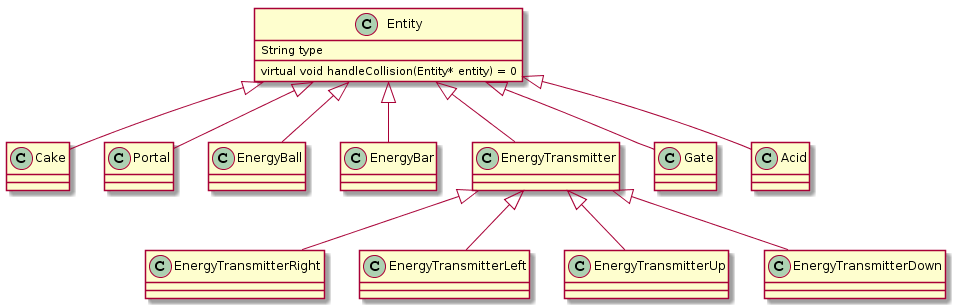
\includegraphics[width=1.5\textwidth]{server_class_1.png}}
	\caption{Diagrama de clases de los elementos del juego}
	\label{fig:diagrama1}
\end{figure}

\begin{figure}[!h]
	\makebox[\textwidth][c]{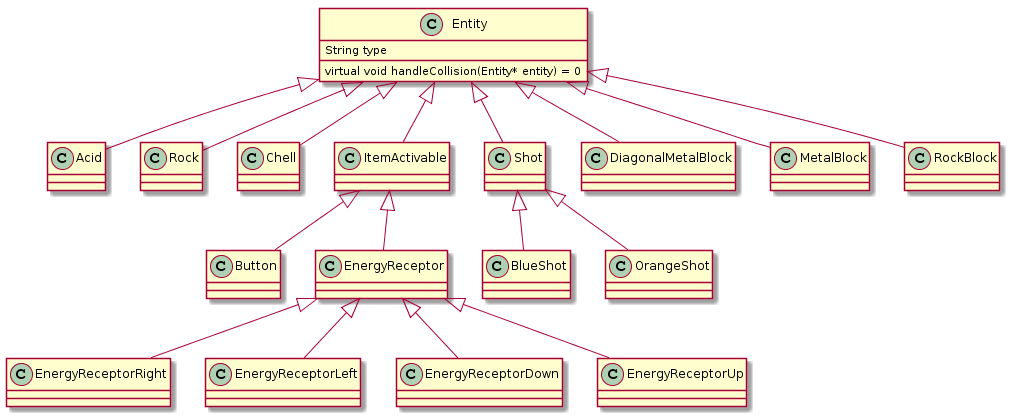
\includegraphics[width=1.5\textwidth]{server_class_2.png}}
	\caption{Diagrama de clases de los elementos del juego}
	\label{fig:diagrama2}
\end{figure}

\newpage
\subsubsection{Manejo de portales}

\begin{figure}[!h]
	\makebox[\textwidth][c]{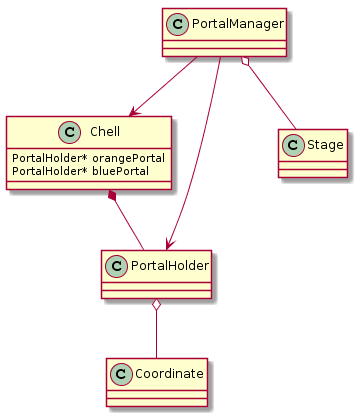
\includegraphics[width=0.6\textwidth]{server_class_3.png}}
	\caption{Diagrama de clases de los elementos utilizados para manejar los portales}
	\label{fig:diagrama3}
\end{figure}

\newpage

\subsubsection{Manejo del escenario}

\begin{figure}[!h]
	\makebox[\textwidth][c]{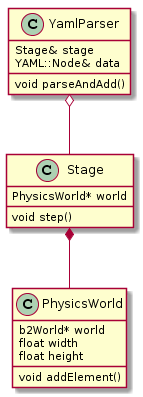
\includegraphics[width=0.25\textwidth]{server_class_4.png}}
	\caption{Diagrama de clases de los elementos utilizados para manejar el escenario}
	\label{fig:diagrama4}
\end{figure}

\newpage

\subsubsection{Soporte de comunicación}

\begin{figure}[!h]
	\makebox[\textwidth][c]{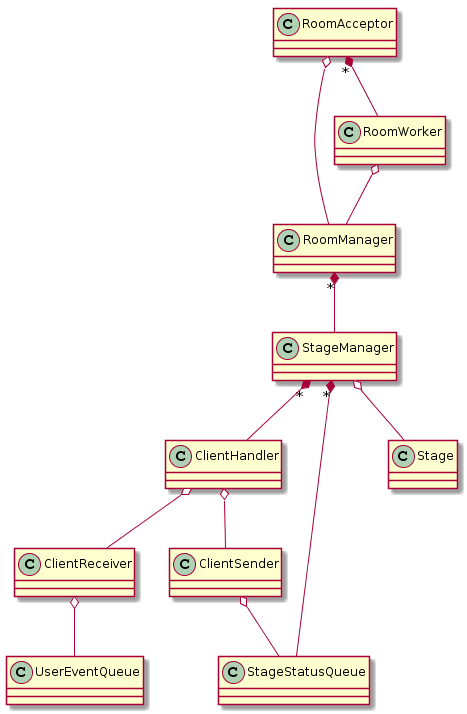
\includegraphics[width=0.75\textwidth]{server_class_5.png}}
	\caption{Diagrama de clases de los elementos utilizados para el soporte de comunicación}
	\label{fig:diagrama5}
\end{figure}

Es pertinente aclarar que no se mostró en el diagrama la relación con la clase \texttt{Protocol} y la clase \texttt{Socket} por claridad.
\newpage

\subsection{Descripción de archivos y protocolos}

El protocolo implementado consistió en enviar y recibir \texttt{strings} por medio de sockets utilizando el protocolo \texttt{TCP}. Estos strings provenían de objetos de la clase \texttt{nlohmann::json}, implementada por la librería \texttt{nlohman} \footnote{https://github.com/nlohmann/json} que tienen un método de conversión a strings. Para el envío de strings se envía primero el largo del string y luego el string. Para recibir simplemente se recibe un string.

La idea utilizada consistió en inicialmente mandar tres jsons de estado:
\begin{enumerate}
	\item Metadata: largo y ancho del escenario:
	\begin{verbatim}
	json[id] = {
		 {"height", height}, {"width", width}
	};
	\end{verbatim}
	\item Data de objetos estáticos (bloques metálicos, bloques en diagonal y bloques de roca):
	\begin{verbatim}
		json[id] = {
			{"type", NAME}, {"x", x}, {"y", y}
	};
	\end{verbatim}
	La constante \texttt{NAME} varia para cada objeto y fue definida en un archivo de uso compartido \texttt{constants.h}.
	\item Data de objetos dinámicos (todo el resto de los objetos). Se trata de los objetos que fueron designados con un id en particular:
	\begin{verbatim}
			json[id] = {
	{"state", state}, {type", NAME}, {"x", x}, {"y", y}
	};
	\end{verbatim}
	Nuevamente la constante \texttt{NAME} se trata de un \texttt{int} definido en el archivo \texttt{constants.h} y el estado se designa de acuerdo al tipo de objeto. Hay objetos que no tienen estado pero la gran mayoría sí:
	\begin{itemize}
		\item Chell: IDLE, JUMPING, MOVING RIGHT, MOVING LEFT
		\item Portal: HORIZONTAL o VERTICAL
		\item Button: ON o OFF
		\item Receptor: ON o OFF
		\item Energy Bar: HORIZONTAL o VERTICAL
		\item Gate: OPEN o CLOSED
	\end{itemize}
\end{enumerate}

Luego, en cada \texttt{step} simulado por \texttt{Box2D} se envía al cliente un \texttt{json} en forma de \texttt{string} como el último descrito, es decir, con la actualización de los objetos dinámicos en el mundo físico.

\section{Cliente}

\subsection{Descripción general}
Las funcionalidades del cliente se dividen en tres partes:
\begin{enumerate}
	\item Las relativas al motor gráfico, es decir, aquellas que sólo se encargan de representar el modelo del juego visual y auditivamente y distintas pantallas a modo de menu.
	\item Las relativas al manejo de sockets para poder comunicarse con un servidor.
\end{enumerate}

A continuación se enumeran las principales clases que se encargan de implementar dichas funcionalidades y sus principales atributos y métodos.

\subsection{Clases}

Para describir las clases utilizadas se dividirán las clases en 3 categorías:

\subsubsection{Soporte para input de usuario}

\begin{itemize}
	\item \textbf{UserEventHandler}
\end{itemize}

Sus atributos principales son una camara \texttt{Camara}, una cola de sonidos \texttt{SoundCodeQueue} y una referencia a una cola de eventos de usuario \texttt{UserEventQueue}. 
Se encarga de procesar eventos de SDL y crear eventos propios \texttt{UserEvent} para encolar en la cola, así como también encolar sonidos a reproducir cuando corresponda (por ejemplo, al disparar).
Estos eventos luego serán consumidos por \texttt{EventSender}.
Esta clase se corre en un thread propio, para poder procesar eventos de SDL sólo si existe uno, en lugar de hacer polling en el thread principal, lo cual además podría impactar la performance de dicho thread ya que allí se dibuja a pantalla, y es crítico mantener una performance aceptable para una mejor experiencia de usuario.

\subsubsection{Soporte para vistas y sonidos}

\begin{itemize}
	\item \textbf{View}
\end{itemize}

Sus atributos principales son una ventana \texttt{Window}, un factor para pasar de unidades de Box2D a pixeles, y una caja de colisión \texttt{SDL\_Rect} para revisar colisiones contra la cámara.
Esta clase es virtual, es decir, ha de ser implementada por cada una de las vistas que representan entidades del modelo.
Cuenta con métodos implementados, los cuales son \texttt{move} para actualizar la posición actual de la vista en pantalla, y \texttt{checkCollisionWithCamera} el cual es utilizado por las vistas para determinar si deben ser dibujadas o no.
El fin de revisar colisión con la cámara es evitar dibujar innecesariamente texturas que el jugador no podrá ver, mejorando la performance del programa.

Los métodos virtuales que han de ser implementados por las clases derivadas son \texttt{playAnimation} y \texttt{setState}. El primero contendrá la lógica para ejecutar las animaciones de cada vista derivada, y el segundo se utiliza para la lógica de cambio de estado de una entidad del modelo, con el fin de representar con mayor fidelidad a las entidades modeladas en el motor físico.

No se describiran la totalidad de las vistas derivadas, sólo la más compleja que es \texttt{ChellView}.

\begin{itemize}
	\item \textbf{ChellView}
\end{itemize}

Esta clase deriva de View. Se encarga de representar en pantalla a nuestro personaje principal.
Entre sus atributos, tenemos un estado actual y un estado previo, esto se utiliza para encolar el sonido del salto en la cola de sonidos. Además cuenta con un timer para saber cuándo encolar un sonido al correr, y otro para saber cuándo dejar de dibujar la animación de muerte.
En el método \texttt{setState}, se actualiza el estado previo y el estado actual con el estado recibido por parámetro.
En el método \texttt{playAnimation} se decide qué animación dibujar, dependiendo del estado actual de Chell. Si Chell está corriendo, se chequea el timer para saber si hay que reproducir un sonido en este estado, el chequeo se encarga de actualizar dicho timer.
En el caso de la muerte, se reproduce la misma durante una cantidad predeterminada de iteraciones.

\begin{itemize}
	\item \textbf{Camara}
\end{itemize}

Esta clase consta de un SDL\_Rect, el cual determinará qué se muestra en pantalla. La misma se centra sobre el jugador asignado al usuario.
Es una clase protegida ya que debió ser utilizada entre dos distintos threads, por lo tanto fue pertinente protegerla para evitar race conditions.

\begin{itemize}
	\item \textbf{ViewManager}
\end{itemize}

Esta clase se encarga de manejar todas las vistas que requieren una actualización de estado, tienen animación o requieren actualizar su posición en el mundo.
Para esto se tiene un mapa donde cada clave es un ID y el valor asociado un puntero a una View. Adicionalmente, cuenta con otro mapa para asociar ID de ChellView con nombre de jugador, para así poder dibujar en pantalla el nombre del jugador sobre su personaje, para poder distinguir entre distintos jugadores.
En cuanto a la actualización del modelo, se consumen JSONs desde una cola diseñada para contener el estado del modelo en dicho formato. La idea principal es que ViewManager sólo actualizará y dibujará aquellas  Views cuyos IDs se hayan recibido en el JSON que contiene la actualización del modelo del juego.
En cuanto a la creación, se recibe inicialmente un JSON con todas las vistas que serán necesarias durante la ejecución del nivel.

\begin{itemize}
	\item \textbf{StageView}
\end{itemize}

Esta clase se encarga de dibujar todos los sprites estáticos que no cambiarán nunca de posición, como por ejemplo los bloques de metal, roca, diagonal, etc.
En cuanto a la creación, se recibe inicialmente un JSON con todos los bloques que serán necesarios durante la ejecución del nivel.
El dibujado de los bloques naturalmente posa un problema importante: Si se dibuja todo el nivel en todo momento, podríamos ocasionar un buffer overflow en el buffer que contiene las texturas dibujadas.
Para evitar este problema, se pensó el diseño de la clase de forma tal que sólo se dibujen aquellos bloques que colisionarían con la cámara. Para esto se guardan los bloques según sus coordenadas, luego se toma el origen de la cámara y se lo transforma a metros.
El paso siguiente es determinar dos rangos para iterar las claves del mapa de bloques, uno en X (se hace con el origen en X de la cámara y el ancho de la misma) y el otro en Y (misma idea pero en Y y con el alto), adicionalmente agregamos algunos bloques extra a modo de borde, para que la transicion entre texturas en la pantalla sea más suave y se obtenga una mejor experiencia de usuario.
Finalmente, sólo dibujamos los bloques que existan en nuestro mapa y cuyas claves (coordenadas)estén dentro de este rango.

\begin{itemize}
	\item \textbf{AudioSystem}
\end{itemize}

Esta clase se encarga de consumir códigos de sonido desde una cola de códigos de sonido, y reproducirlos.
Los sonidos se guardan en un mapa donde tenemos como clave un código de sonido, y como valor asociado un \texttt{Mix\_Chunk*} el cual contiene el sonido a reproducir.
Adicionalmente, contamos con un mapa similar pero para música. En la implementación actual del TP no fue utilizado en todo su potencial este feature, pero en próximos releases agregaremos más canciones y la posibilidad de cambiar de música en medio de la partida.

\begin{itemize}
	\item \textbf{Game}
\end{itemize}

Esta clase se encarga del flujo previo al inicio de una partida, es decir, creación/unión de partida.
Cuenta con clases para representar las pantallas de unión/creación de partida, selección de nivel, selección de nombre de jugador.

\begin{itemize}
	\item \textbf{Drawer}
\end{itemize}

Esta clase contiene a las clases necesarias para poder dibujar el modelo del juego en pantalla, así como también realizar la comunicación con un servidor dado.
Aquí encontramos el game loop, en donde consumimos el estado actual del modelo enviado por el servidor, a través de una cola bloqueante. Si no hay un estado nuevo, simplemente utilizamos el estado anterior para dibujar, de esta forma evitamos cortar el dibujado en caso de alta latencia.

\subsubsection{Soporte para comunicación}

\begin{itemize}
	\item \textbf{Event Sender}
\end{itemize}

Sus atributos son un protocolo \texttt{Protocol} y una referencia a una cola de eventos de usuario \texttt{UserEventQueue}. Se encarga de enviar los diversos eventos de usuario al servidor, por medio del protocolo que encapsula el envío a través de sockets.

\begin{itemize}
	\item \textbf{State Status Receiver}
\end{itemize}

Sus atributos son un protocolo \texttt{Protocol} y una referencia a una cola de estados del escenario \texttt{StageStatusQueue}. Se encarga de recibir los diversos estados del escenario, enviados por el servidor, para dibujar los elementos dinámicos en su estado actual.

\newpage

\subsection{Diagramas UML}

\subsubsection{Soporte para vistas y sonidos}

\begin{figure}[!h]
	\makebox[\textwidth][c]{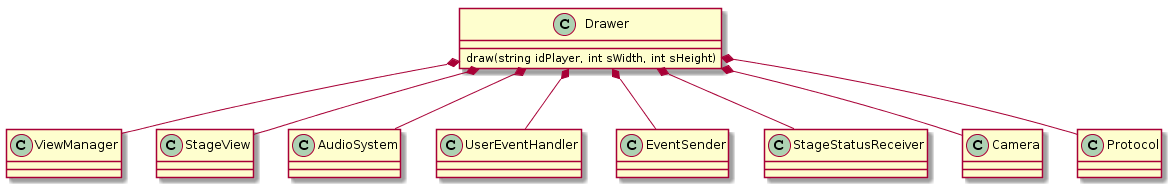
\includegraphics[width=1.5\textwidth]{umlDrawer.png}}
	\caption{Diagrama de clases del soporte para vistas y sonidos}
	\label{fig:diagram6}
\end{figure}

\begin{figure}[!h]
	\makebox[\textwidth][c]{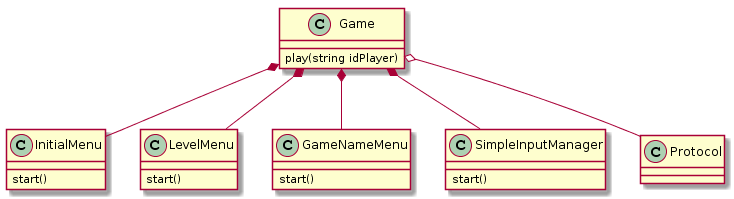
\includegraphics[width=1.25\textwidth]{umlGame.png}}
	\caption{Diagrama de clases del soporte para vistas y sonidos}
	\label{fig:diagram7}
\end{figure}


\begin{figure}[!h]
	\makebox[\textwidth][c]{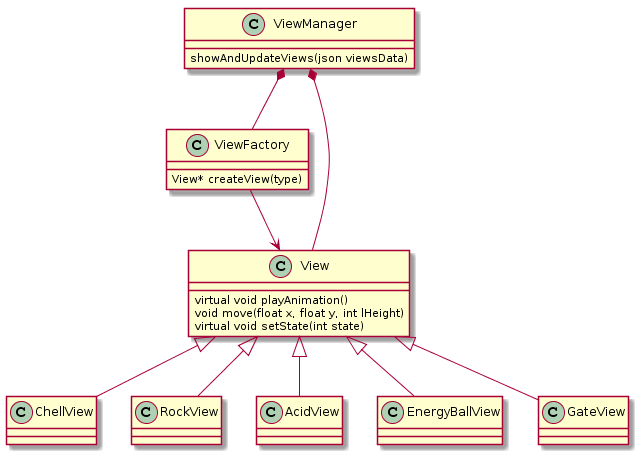
\includegraphics[width=1.3
		\textwidth]{umlViewManager.png}}
	\caption{Diagrama de clases del soporte para vistas y sonidos}
	\label{fig:diagram8}
\end{figure}


\begin{figure}[!h]
	\makebox[\textwidth][c]{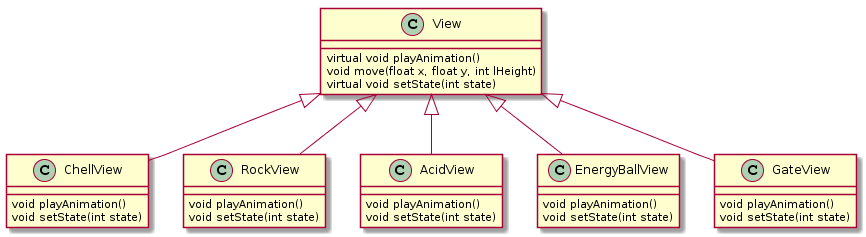
\includegraphics[width=1.6\textwidth]{umlViews.png}}
	\caption{Diagrama de clases del soporte para vistas y sonidos}
	\label{fig:diagram9}
\end{figure}

\newpage

\subsubsection{Soporte para comunicación}


\begin{figure}[!h]
	\makebox[\textwidth][c]{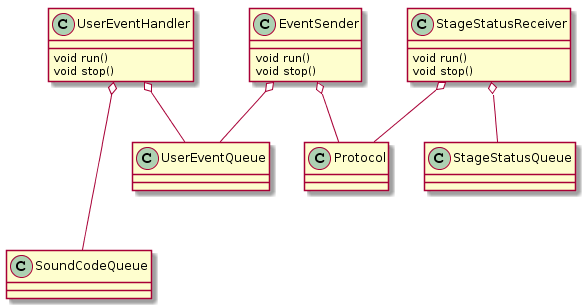
\includegraphics[width=1\textwidth]{client_class_1.png}}
	\caption{Diagrama de clases del soporte de comunicación del cliente}
	\label{fig:diagram10}
\end{figure}

\subsection{Descripción de archivos y protocolos}

Contamos con un archivo de configuración para setear la resolución de la ventana de juego, y del factor utilizado para convertir unidades de Box2D a pixeles. Es importante que la resolución sea múltiplo de este factor, para así obtener una transición suave entre texturas al mover la cámara.

Como ya se mencionó en la sección del servidor, se utiliza el formato JSON para el envío y recepción de información.

Adicionalmente a los requests ya descriptos en la sección del servidor, contamos con los siguientes requests:

\begin{enumerate}
	\item Lista de juegos:
	\begin{verbatim}
	{ "games":
		 ["Aprueben", "este", "tp", "por favor"]
	};
	\end{verbatim}
	\item Creación o unión:
	\begin{verbatim}
	{ "action": CREATE_GAME_CODE
	};
	\end{verbatim}
	Donde CREATE\_GAME\_CODE y JOIN\_GAME\_CODE son enteros, 0 y 1 respectivamente.
	\item Campos de partida y ID jugador:
	\begin{verbatim}
	{ "game": gameName,
	  "id": somePlayerName
	};
	\end{verbatim}
	\item Resultado de la acción procesada en el servidor:
	\begin{verbatim}
	{ "result": SUCCESS_CODE,
	  "idChell": Chell1
	};
	\end{verbatim}
	El campo "result" puede ser SUCCESS\_CODE o FAIL\_CODE, dependiendo de si salió todo bien o no. "idChell" es el ID asignado por el servidor a la Chell del jugador.
	\item UserEvent enviado al servidor:
	\begin{verbatim}
	{ "id": userId,
	  "eventType": eventTypeCode,
	  "x": mousePositionX,
	  "y": mousePositionY
	};
	\end{verbatim}
	Este request contiene toda la información que necesita el servidor para poder procesar un evento de usuario. X e Y respectivamente se dejan en 0 si el evento no requiere saber estos valores.
	EventTypeCode es un entero con distintos valores, el listado completo puede observarse en el archivo \texttt{common/constants.h}
\end{enumerate}

\section{Editor}

\subsection{Descripción general}

Las funcionalidades del servidor se dividen en dos partes:
\begin{enumerate}
\item El menú donde el usuario podrá ver los distintos elementos que son posibles agregar al escenario.
\item El escenario el cual el usuario podrá editar e ir viendo su progreso.
\end{enumerate}

\subsection{Clases}

\subsubsection{Editor}

El Editor es una suerte de “manejador” del Stage y Menu. Se encarga de recibir los handles de SDL y articular entre ambas clases según sea necesario.

\subsubsection{Menu}

El objetivo principal de esta clase es mostrar todos los posibles elementos en pantalla y actualizar la referencia al objeto seleccionado. Es decir, que cada vez que el usuario hace un click en alguna de las opciones proporcionadas el Menu guarda en una variable compartida el ID de este objeto.

\begin{itemize}
\item \textbf{MenuButton}
\end{itemize}

Esta clase es utilizada por el Menu para instanciar las distintas opciones. Cada uno de los elementos visibles en el menú es una instancia de esta clase con una imagen específica. Su principales labores son dibujarse y verificar si el handle detectado se dio dentro de ellos para así brindar el ID de la opci+on que representan.

\subsubsection{Stage}

La funcionalidad principal del stage es manejar todos los pedido provenientes del Editor para ello debe:
\begin{enumerate}
\item Verificar que realmente el evento generado por el usuario se encuentre dentro del escenario.
\item Ejecutar el handle. En punto en general consta de enviarle una instrucción al Controller.
\end{enumerate}

\begin{itemize}
\item \textbf{Controller}
Esta clase cuenta con:
\begin{enumerate}
\item Referencia a todas las posibles opciones ID a agregar y un puntero a una instancia real de lo que ese ID representa (`Object*`).
\item Una lista de tipo clave-valor de todas las posiciones del escenarios (como clave) y el ID del objeto que ocupa ese lugar (como valor).
\item Una instancia de View.
\item Una instancia de LogicGates.
\item Una instancia de YamlManager.
\end{enumerate}

El controlador inicialmente se encargaba únicamente de agregar y sacar elementos del mapa. A través de los últimas 3 atributos el controller pudo deriva parte de sus nuevas funcionalidades. Las mismas son: dibujar el mapa que se está editando, nombrar los objetos que pueden ser nombrados (botones, receptores, compuertas) agregar condiciones lógicas a las compuertas y leer y escribir archivos de tipo `.yaml`. En conclusión el controlador es el encargado de manejar todos los aspectos del escenario.

\item \textbf{LogicGates}

Esta clase tiene una referencia a todos los objetos que pueden ser nombrados (en el modelo actual son sólo 3) y todos los objetos que conllevan una condición lógica (en el modelo actual existe sólo 1). Su funcion principal es comunicarse con el usuario por la pantalla y asi pedirle un string para poder almacenarlo en el objeto que corresponda.

\item \textbf{YamlManager}

Esta clase conoce perfectamente el manejador de archivos de extención `.yaml` así como las necesidades del servidor. Es decir, se encarga de escribir un archivo de forma tal que pueda ser interpretado por este. Ademas el mismo tiene la capacidad de interpretar el archivo que produce y de setear un enescenario en edición a partir del mismo. Es menester que el YamlManager conozca al LogicGates intanciado por el Controller porque es necesario plasmar en el archivo de salida las condiciones lógicas ingresadas por el usuario.


\item \textbf{View}

Esta clase se encarga de dibujar el mapa completo. La implementación del controller facilita que el escenario sea infinito sin ningún problema de performance. Para que este feature sea visible al usuario es esencial que esta clase sepa plasmar el movimiento del movimiento del mapa. Esto es posible ya que a la hora de ser dibujado recibe como parámetro un SDLRect* que indica la posición de la cámara con respecto a los objetos del escenario.

\item \textbf{Object clase base}

Los objetos y su polimorfismo son esenciales para la implementación de este modelo. Cada objeto tiene su alto y ancho y su propio id. Además los objetos saben cuando pueden agregarse o quitarse del escenario. Así como calcular su centro de masa a partir de una posición en una matriz y viceversa.

\item \textbf{Object clases derivadas}

Las clases derivadas se encargan de sobrescribir ciertos comportamiento en los que difieren de la clase madre. Por ejemplo, StacticObjects y AnimatedObject sobrescriben la forma de dibujarse.

\end{itemize}

\subsection{Diagramas UML}
Se procede a exponer los diagramas de clase realizados para las diversas secciones.

\newpage

\subsubsection{Clases principales}

\begin{figure}[!h]
\makebox[\textwidth][c]{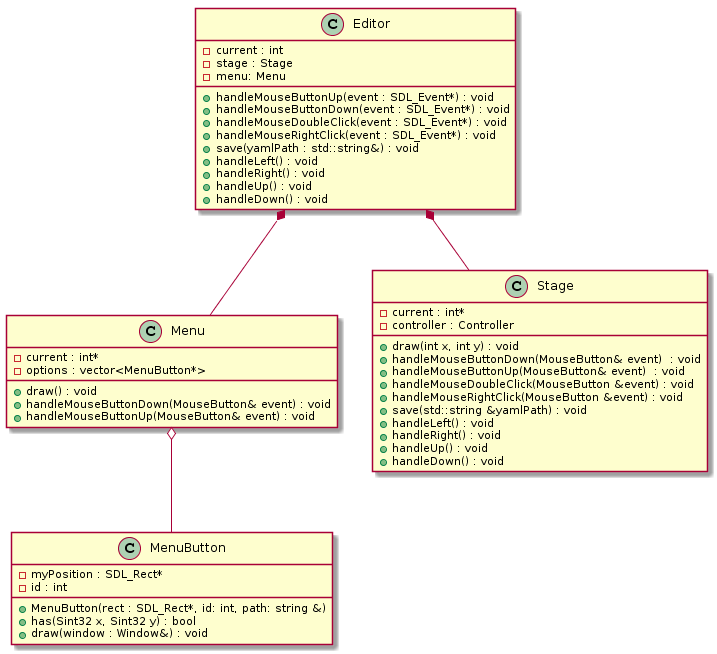
\includegraphics[width=1.5\textwidth]{editor_clases_basico.png}}
\caption{Diagrama de clases más abarcativas del editor}
\label{fig:diagrama5}
\end{figure}

\newpage
\subsubsection{Modelo del stage}

\begin{figure}[!h]
\makebox[\textwidth][c]{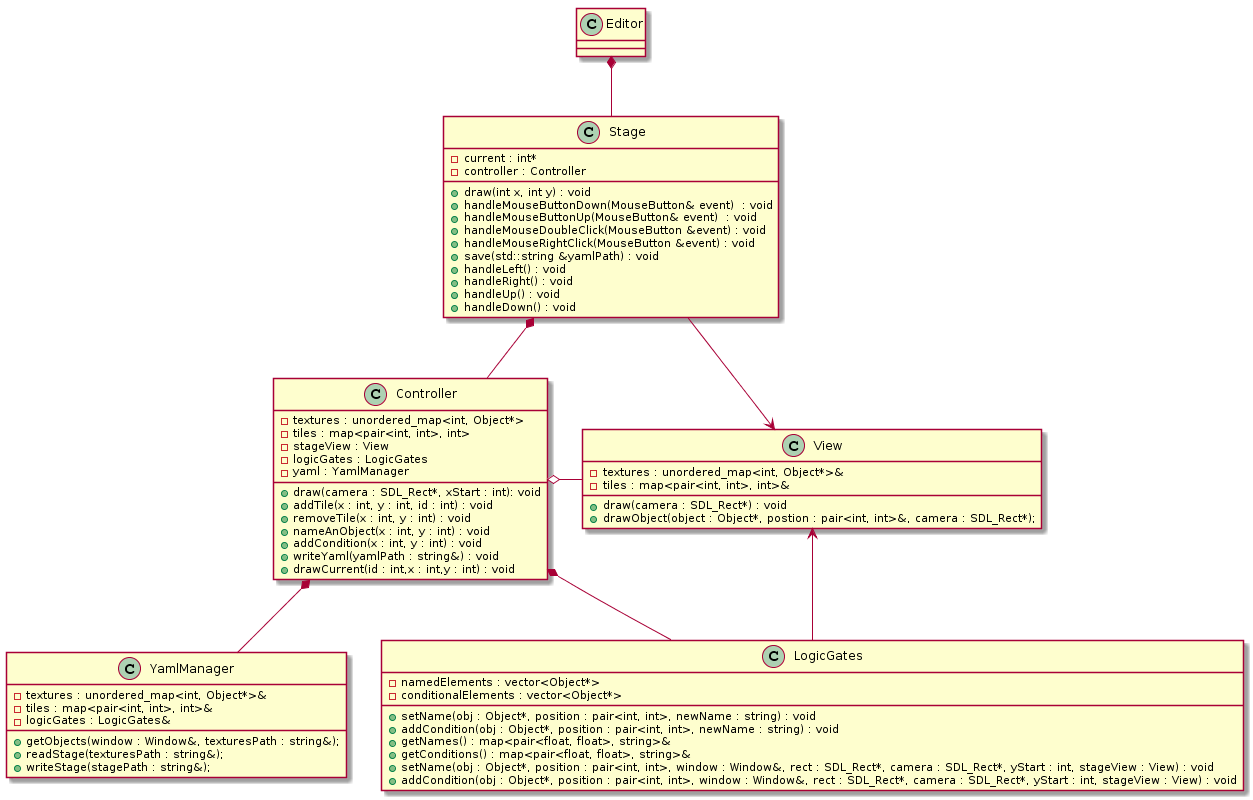
\includegraphics[width=1.5\textwidth]{editor_stage_zoom.png}}
\caption{Diagrama de clases más funcionales del editor}
\label{fig:diagrama6}
\end{figure}

\newpage
\subsubsection{Objetos del escenario}

\begin{figure}[!h]
\makebox[\textwidth][c]{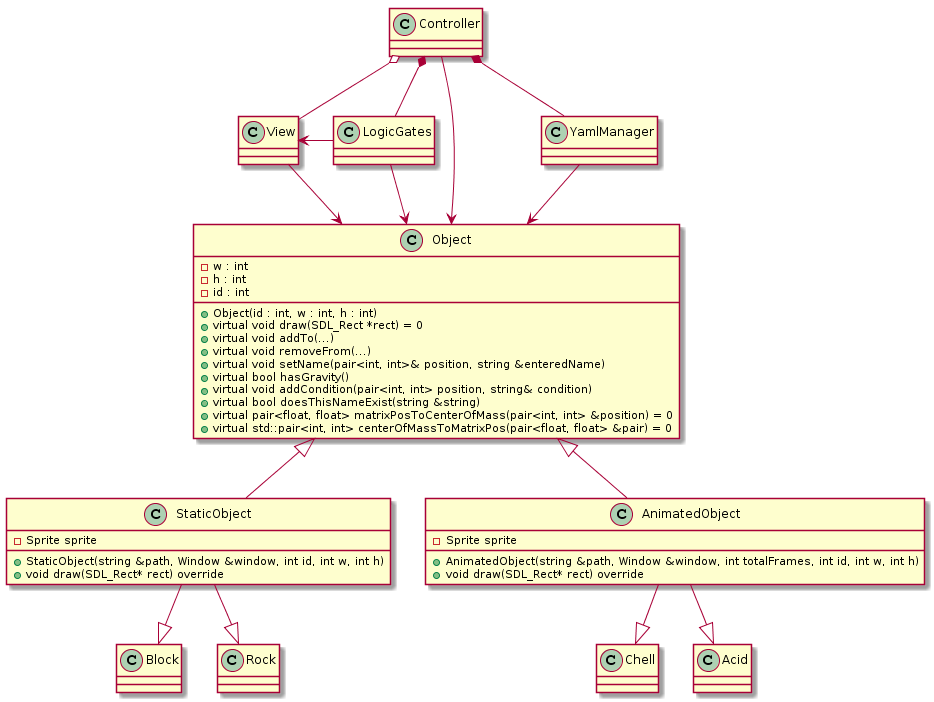
\includegraphics[width=1.5\textwidth]{editor_object_zoom.png}}
\caption{Diagrama de clases más especificas del editor}
\label{fig:diagrama7}
\end{figure}


\end{document}